\Huge\textbf{Capitolo 2: \\ Struttura e funzioni delle proteine}

\section{Struttura gerarchica}
    \small
    L'intero insieme di proteine che può essere espresso da una data cellula prende il nome di \textbf{proteoma}. Il genoma consente di identificare molte più proteine rispetto a quelle effettivamente espresse.\\
    Le proteine sono enormemente eterogenee e hanno funzioni molto diverse. Si classificano in:
    \begin{itemize}
        \item dipeptidi: composti da due amminoacidi (AA)
        \item peptidi: composti da pochi AA (maggiori di 2)
        \item oligopeptidi: composti da meno di 20/30 AA
        \item polipeptidi: composti da 200/500 AA 
    \end{itemize}
    I 20 AA di cui si compongono le proteine si dividono nelle seguenti categorie:
    \begin{itemize}
        \item non polari
        \item polari, che a loro volta si dividono in: 
        \begin{itemize}
            \item carichi positivamente
            \item carichi negativamente
            \item neutri
        \end{itemize}
    \end{itemize}
    Gli AA sono legati l'un l'altro tramite legami peptidici (covalenti), la reazione che porta al legame è una reazione di consensazione. Abbiamo una catena di atomi del backbone sempre uguale a se stesso (NCC...NCC). Il primo C è il carbonio $\alpha$ a cui è legata la catena laterale R.\\
    La catena amminoacidica si legge a partire dall'AA che espone l'N-terminale (amminoterminale) fino all'AA che espone il C-terminale (carbossiterminale) perchè corrisponde all'ordine di sintesi del peptide, da qui la sua polarità.\\
    Ogni proteina sintetizzata assume una conformazione tridimensionale dovuta alle interazioni elettrostatiche tra gli AA. L'urea è una molecola che destabilizza la formazione di questi legami. Ci sono enzimi (chaperon) che concorrono alla formazione della conformazione tridimensionale corretta.\\
    Le combinazioni degli stretch di AA sono teoricamente infinite, ciononostante, le proteine realmente prodotte fanno parte di un range molto più ristretto e quindi non ogni combinazione di AA viene realizzata. La diversità strutturale è ancora minore, in quanto esiste un numero relativamente più limitato di conformazioni. 
    Per esempio alcuni tratti della sequenza di elastasi e chimotripsina sono simili se non identici. Formano entrambe una conformazione molto simile e sono coinvolte entrambe nella digestione delle proteine.
          \begin{figure}[h]
            \centering
            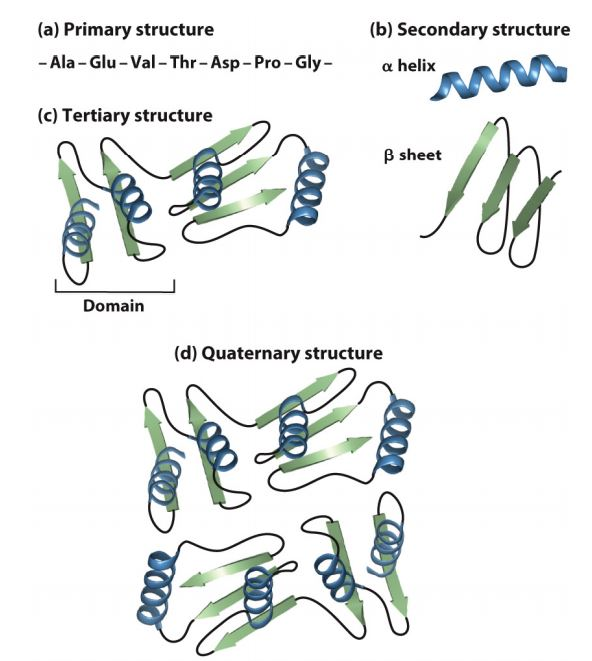
\includegraphics[width=0.5\textwidth]{images/proteinegerarchia.JPG}
            \caption{\small schema generale delle strutture proteiche}
            \label{fig:mesh1}
        \end{figure}
    
    \subsection{Folding}
        Per \textbf{Folding} si intende il processo di ripiegamento della catena amminoacidica per la formazione della propria \textit{conformazione} (dettata dalla sequenza di AA). 
        Questo evento consiste nella formazione di legami non covalenti (legami a idrogeno, interazioni di van der Waals e interazioni idrofobiche) tra le catene laterali degli AA o il backbone della catena amminoacidica stessa (tutte le combinazioni sono possibili).\\
        La base che consente il ripiegamento è il fatto che i due legami che interessano il carbonio $\alpha$ hanno una determinata libertà rotazionale (al contrario del C del legame peptidico).\\
        Nel caso di una proteina denaturata, il processo di folding avviene spontaneamente.\\
        Le ripiegature scorrette possono essere la causa di patologie (per esempio il morbo della mucca pazza).
        \subsubsection{Eccezioni}
            In alcuni casi il folding può avvenire tramite interazioni covalenti tra catene polipeptidiche diverse o dello stesso polipeptide.\\
            
            \textbf{Ponte di-solfuro}  \\
                Il ponte di solfuro si forma su due cisteine (legame covalente), che consolidano interazioni non-covalenti all'interno della cellula cosicché possa mantenere la stessa stabilità e conformazione all'esterno.\\
                Esempio: in un anticorpo, le catene pesanti e leggere presentano ponti di-solfuro tra per stabilizzare la molecola (sia interni alla stessa catena sia tra catene diverse). 
                La specificità dell'anticorpo è determinata da anse iper-variabili che legano l'antigene ed è funzionale solamente se la struttura quaternaria è corretta (i ponti di-solfuro sono necessari per questo motivo).
    
    \subsection{Struttura primaria}
        La struttura primaria della proteina consiste nella sequenza amminoacidica di cui è composta, è polarizzata (ovvero ha una direzione N - C) e si considera il primo AA quello che espone l'N-terminale.
    
    \subsection{Struttura secondaria}
        La struttura secondaria consiste in ripiegamenti locali della sequenza di AA. Le due strutture secondarie principali che si riscontrano sono $\alpha$-Elica ($\alpha$E) e $\beta$-Foglietto (F$\beta$). \\
        Glicina e prolina hanno la minore propensione di essere coinvolte in una struttura $\alpha$E o F$\beta$.
        \subsubsection{$\alpha$-Elica}
            L'$\alpha E$ è un organizzazione 3D che consiste nella disposizione dei residui AA verso l'esterno, è resa stabile per i legami H tra gli atomi del backbone, il quale ha una conformazione elicoidale. 
            La sua struttura risulta sempre uguale a se stessa indipendentemente dai residui AA (un O si lega sempre ad un H dell'AA quattro posizioni più avanti). Il passo dell'elica corrisponde a 0.54 nm. Per compiere un giro sono necessari 3.6 AA.\\
            Alcuni AA interferiscono con la formazione della struttura, in particolare glicina e prolina.\\
            L'$\alpha E$ può assumere proprietà chimiche differenti a seconda della sequenza AA che la compone. 
            Per esempio può contenere code idrofobiche nel caso l'$\alpha E$ sia destinata a fare parte di un complesso proteico trans-membrana.\\
            Può essere destrorsa o sinistrorsa, la maggioranza delle eliche in natura è destrorsa.
        
        \subsubsection{$\beta$-Foglietto}
            Il $\beta F$ è basato sulle interazioni H tra gli atomi del backbone. Le catene laterali degli AA sono disposte alternativamente sopra e sotto il piano del foglietto. Anche in questo caso, la sua struttura è indipendente dalla catena AA ed è sempre uguale a se stessa, le catene laterali non sono coinvolte. \\
            Gli \textit{strand} planari del foglio possono essere orientati relativamente in maniera:
            \begin{itemize}
                \item parallela (da un lato del foglietto si trovano tutti gli N-terminali), connesso da loop più ampi
                \item antiparallela (l'N-terminale si alterna tra i lati del foglio). 
                Viene chiamato $\beta$-turn il ripiegamento che connette due filamenti antiparalleli, ha una composizione sistematica di 4 AA (spesso sono presenti glicina e prolina)
            \end{itemize}
            Esistono strutture ibride (porzioni parallele e antiparallele).
    
    \subsection{Struttura terziaria}
        Per struttura terziaria si intendono ripiegamenti dell'intero polipeptide.\\
        Un \textit{motivo strutturale} non è propriamente una struttura terziaria ma è un intermedio precedente alle strutture terziarie vere e proprie.\\
        Anche il \textit{dominio} è un intermedio precedente della struttura terziaria, ovvero un ripiegamento di una porzione di AA a sè stante.
        \subsubsection{Coled-coil motiv}
            La struttura del Coiled-coil è un motivo molto presente in proteine fibrose e si può formare in presenza di due $\alpha E$ che si "arrotolano" su loro stesse. \\
            Le eliche che tendono a formare questa struttura comprendono delle sequenze AA specifiche chiamate \textit{heptad repeat} lunghe sette AA. 
            Le posizioni interne a questa sequenza sono spesso indicate con \textit{abcdefg} dove tipicamente \textit{a} e \textit{d} sono AA idrofobici (1 e 4), quindi un lato di queste eliche risultano idrofobiche.
            Le due eliche, avendo caratteristiche simili, tendono ad associarsi per stabilizzarsi. Non si ripiegano necessariamente l'una sull'altra autonomamente.
        
        \subsubsection{Domini}
            Un dominio è una porzione della proteina che comprende più strutture secondarie e assumono una conformazione autonomamente, un ripiegamento più ampio della struttura proteica. Il dominio si forma autonomamente, la sua conformazione prescinde dal resto dei peptidi.\\
            Uno stesso peptide è solitamente composto da domini differenti (posizioni e possibilmente funzioni diverse).
        
        \subsubsection{Domini non strutturati}
            Un dominio non strutturato non assume conformazione propria perchè sono intrinsecamente disordinate, ma possono interagire con altre molecole conformate (\textit{chaperon}) per assumere una conformazione specifica.\\ 
            Possono svolgere una funzione di signaling o regolatoria.\\
            
            \textbf{Chaperon}\\
                Il folding di una proteina avviene infatti contemporaneamente alla sintesi, qualora la conformazione 3D attesa debba passare attraverso uno stato energicamente sfavorito, può intervenire uno \textit{Chaperon}, che collabora alla formazione della proteina matura e velocizza il processo. 
                Uno chaperon è un enzima che riesce ad abbassare il picco energetico sfavorevole.\\
                Solitamente viene speso ATP cellulare per completare il ripiegamento. Alcuni chaperon forniscono un microambiente che favorisce il ripiegamento oppure possono associarsi alla proteina target nello stesso ambiente.
        
    \subsection{Struttura quaternaria}
        Per struttura quaternaria si intende l'associazione di più polipeptidi per la formazione di un complesso funzionale (non necessaria ma succede spesso).\\
        I polimeri che destinati a formare una struttura quaternaria, non sono spesso in grado di esercitare la propria funzione se lasciati a se stessi.\\
        Le associazioni tra polipeptidi differenti avvengono attraverso legami non-covalenti per la formazione di polimeri. Esistono degli agenti che permettono l'aggregazione di una molecola funzionante.\\
        Nel caso dell'emoglobina, sono presenti quattro polipeptidi (due catene $\alpha$ e due $\beta$), solamente se associata nella conformazione corretta compie la sua funzione. A livello evolutivo si trovano sequenze omologhe all'emoglobina e si trovano proteine simili con funzioni analoghe in organismi molto distanti.\\
        Ci sono anche associazioni sopramolecolari di proteine per la formazione di un complesso funzionale, ad esempio il ribosoma.
    
\section{Funzioni}
    Le funzioni delle proteine possono essere talvolta già associate ad una struttura terziaria. In alcuni casi il ruolo di un polipeptide è funzionale ad un complesso strutturalmente più complesso (ad esempio il ribosoma). \\
    Le funzioni principali delle proteine sono:
    \begin{enumerate}
        \item regolatoria
        \item strutturale
        \item movimento della cellula
        \item enzimatica
        \item trasporto
        \item signaling
    \end{enumerate}
    
\pagebreak